\documentclass{standalone}
\usepackage{tikz}
\usepackage{amsmath}
\usepackage{pgfplots}

\begin{document}
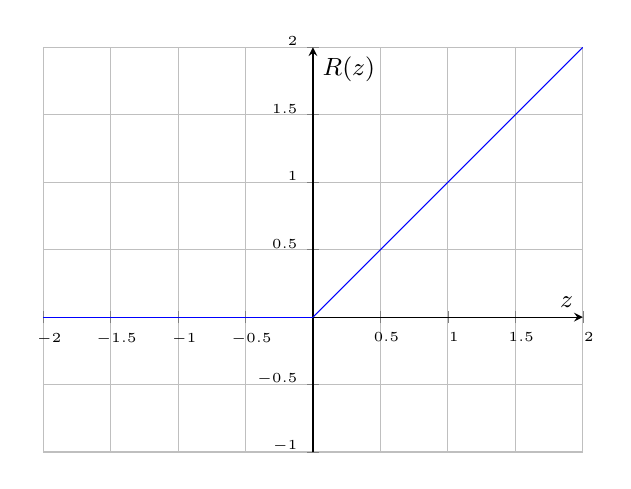
\begin{tikzpicture}[font=\small]
    % \draw[->] (-3.5,0) -- (3.5,0) node[right] {$x$};
    % \draw[->] (0,-1.2) -- (0,3.5) node[above] {$f(x)$};
    % \draw[scale=1,domain=0:3,smooth,variable=\x,blue] plot ({\x},{\x});
    % \draw[scale=1,domain=-3:0,smooth,variable=\x,blue] plot ({\x},{0});
    \begin{axis}[
    unit vector ratio*=1 1 1,
            legend pos=north west,
            xmin=-2, xmax=2, ymin=-1, ymax=2, grid=both,
            ylabel={$R(z)$}, xlabel={$z$},
            xtick={-2,-1.5,...,2}, ytick={-2,-1.5,...,2},
            xticklabel style={font=\tiny, xshift=0.5ex},
            yticklabel style={font=\tiny, yshift=0.5ex},
            axis line style={->},
            axis x line=middle,
            axis y line=middle,
        ]
        \addplot+[mark=none, color=blue, domain=0:2] {x};
        \addplot+[mark=none, color=blue, domain=-2:0] {0};
        \end{axis}
        
        
\end{tikzpicture}
\end{document}

